\documentclass[10pt]{beamer}
\mode<presentation>
\setbeamertemplate{bibliography item}{}
\usepackage{beamerthemesplit}
\usepackage{graphicx}
\usepackage{booktabs}
\usepackage{amsmath}
\usepackage{textpos}
\usepackage{pgfplots}
\usepackage{tikz}
\usepackage{hyperref}
\usepackage{caption}
\usetikzlibrary{shapes.geometric, arrows}
\usetikzlibrary {datavisualization} 
\pgfplotsset{compat=1.18, width = 7cm}
\usetikzlibrary{patterns}
\setbeamertemplate{bibliography item}[text]
\usetheme{Ilmenau} % AnnArbor, Ilmenau, Darmstadt, Dresden, CambridgeUS, Frankfurt, Singapore
\newtheorem{dn}{Định nghĩa}[section]
\newtheorem{dl}{Định lý}[section]
\newtheorem{tc}{Tính chất}[section]
\newtheorem{hq}{Hệ quả}[section]
\newtheorem{bd}{Bổ đề}[section]
\newtheorem{md}{Mệnh đề}[section]
\newtheorem{vd}{Ví dụ}[section]
\newtheorem{nx}{Nhận xét}[section]
\newcommand{\dom}{\text{{\rm dom}}}
\newcommand{\epi}{\text{{\rm epi}}}
\newcommand{\Min}{\text{{\rm Min}}}
\setbeamertemplate{theorems}[numbered]
\setbeamertemplate{definitions}[numbered]
\setbeamertemplate{footline}[frame number]
\usepackage{algorithm}
\usepackage{color}
\usepackage{algorithmic}
\usepackage{footmisc}
\usepackage{indentfirst} 
\usepackage{comment}
\AtBeginEnvironment{proof}{%
  \setbeamercolor{block title}{use=example text,fg=white,bg=example text.fg!75!black}
  \setbeamercolor{block body}{parent=normal text,use=block title example,bg=block title example.bg!10!bg}
}
\renewcommand{\thefootnote}{\arabic{footnote}}
\usefonttheme{professionalfonts}
\setbeamercolor{normal text}{bg=white,fg=black}
\renewcommand{\thefootnote}{\arabic{footnote}}
\beamertemplatetransparentcoveredhigh
\usetheme[progressbar=frametitle]{metropolis}
\usepackage{appendixnumberbeamer}

\usepackage[utf8]{vietnam}

\usepackage{booktabs}
\usepackage[scale=2]{ccicons}

\usepackage{pgfplots}
\usepgfplotslibrary{dateplot}

\usepackage{xspace}
\newcommand{\themename}{\textbf{\textsc{metropolis}}\xspace}
\definecolor{mSybilaRed}{HTML}{990000}

\setbeamercolor{title separator}{
  fg=mSybilaRed
}

\setbeamercolor{progress bar}{%
  fg=mSybilaRed,
  bg=mSybilaRed!90!black!30
}

\setbeamercolor{progress bar in section page}{
  use=progress bar,
  parent=progress bar
}

\setbeamercolor{alerted text}{%
  fg=mSybilaRed
}

\setbeamertemplate{footline}
{
  \leavevmode
  \hbox{
  \begin{beamercolorbox}[wd=.15\paperwidth,ht=2.25ex,dp=1ex,center]{title in head/foot}
    \usebeamerfont{author in head/foot}\insertshortauthor
  \end{beamercolorbox}

  \begin{beamercolorbox}[wd=.7\paperwidth,ht=2.25ex,dp=1ex,center]{author in head/foot}
    \usebeamerfont{author in head/foot}\insertshorttitle
  \end{beamercolorbox}

  \begin{beamercolorbox}[wd=.15\paperwidth,ht=2.25ex,dp=1ex,center]{title in head/foot}
    \insertframenumber{} / \inserttotalframenumber
  \end{beamercolorbox}
  }
}


\title{Phương pháp giải bài toán Tối ưu tuyến tính nguyên}


\titlegraphic{\hfill 
\includegraphics[height=1cm]{logodhsg.png}}
%\titlegraphic{\hfill
\includegraphics[height=0.6cm]{sybila-logo/new.png}}
%\titlegraphic{\hfill
\includegraphics[height=0.6cm]{sybila-logo/old.png}}
%\titlegraphic{\hfill
\includegraphics[height=0.6cm]{sybila-logo/old-flat.png}}

\date{\today}
\author{Thực hiện: Đỗ Ngọc Minh Thư, Nguyễn Chí Bằng}
\institute{Sinh viên lớp: DTU1221, Khóa: 22 @ Đại học Sài Gòn}

%\title{Metropolis}
\subtitle{Hướng dẫn: PGS.TS. Tạ Quang Sơn}
% \date{\today}
%\date{}
%\author{Matthias Vogelgesang}
%\institute{Center for modern beamer themes}
%\titlegraphic{\hfill
\includegraphics[height=1.5cm]{logo.pdf}}

\begin{document}
\begin{frame}
  \centering
  {\footnotesize
  ỦY BAN NHÂN DÂN THÀNH PHỐ HỒ CHÍ MINH\\
  TRƯỜNG ĐẠI HỌC SÀI GÒN}\\
  \phantom{space}\\
  {\normalsize BÁO CÁO ĐỀ CƯƠNG NGHIÊN CỨU KHOA HỌC\\
  NGÀNH: TOÁN ỨNG DỤNG}\\[-50pt]
  \titlepage
\end{frame}

\begin{frame}
    \frametitle{NỘI DUNG BÁO CÁO}
    \tableofcontents
\end{frame}

% Tai sao quan tam de tai?
% Lam duoc gi?
% Hoc duoc gi ?
% Du dinh tiep theo ?
% - - -
% Cơ sở lý thuyết và Mục tiêu
\section{Giới thiệu}

\begin{frame}{\bf Mục đích nghiên cứu}
\textbf{Tối ưu tuyến tính} là một nội dung quan trọng trong chương trình đào tạo Cử nhân Toán ứng dụng. Lý thuyết về việc giải bài toán tối ưu tuyến tính đã được cung cấp cho sinh viên. Tuy vậy, có nhiều bài toán tối ưu cần được giải với nghiệm nguyên. Chẳng hạn như:
\begin{itemize}
\item Bài toán tối ưu nhân lực.
\item Bài toán tối ưu vận chuyển hàng hóa.
\item Bài toán tối ưu áp dụng trong tin học.
\end{itemize}

\bigskip
Có một lý thuyết riêng cho việc xử lý các bài toán Tối ưu tuyến tính và \textcolor{red}{tìm nghiệm nguyên.}
\bigskip

{\it Mục đích của đề tài này là tìm hiểu một số phương pháp giải bài toán Tối ưu tuyến tính và tìm nghiệm nguyên cho bài toán.}  
\end{frame}

\begin{frame}{\bf Tại sao cần có một lý thuyết riêng cho bài toán Tối ưu tuyến tính nguyên}

\begin{columns}
    \begin{column}{0.5\textwidth}
        \begin{equation*}
        \begin{array}{lll}            
        {\rm Max}&f(x)=2x_1+2x_2\\
        & \begin{cases}
        2x_1+x_2 \leq  8 \\
        x_1+3x_2 \leq 10 \\
        x_i\geq 0,\forall i=1,2.
        \end{cases} 
        \end{array}
        \end{equation*}
    \end{column}

    \begin{column}{0.5\textwidth}
        \begin{figure}
        \centering
        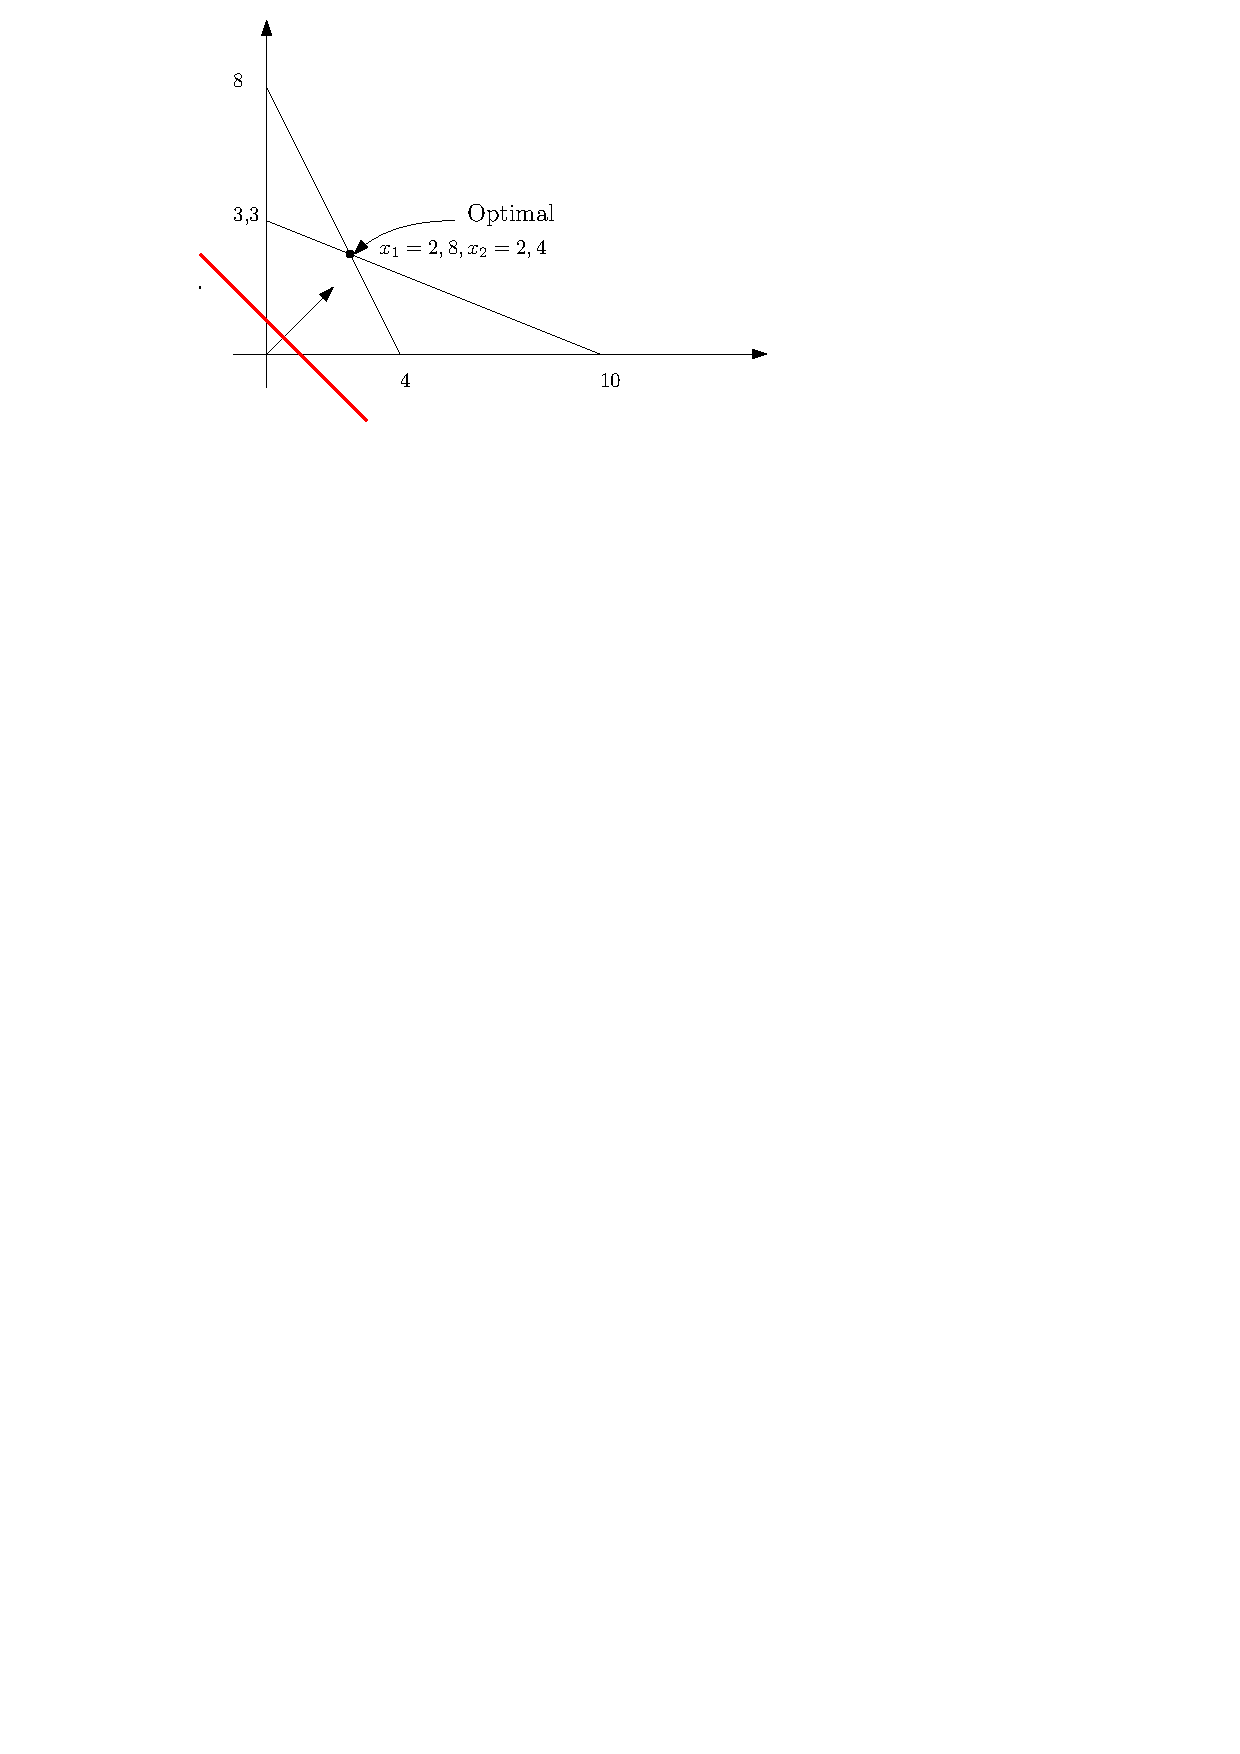
\includegraphics[width=1\linewidth]{Nhom1_hinh.pdf}
        \caption{Hình minh hoạ bài toán}
        \end{figure}
    \end{column}
\end{columns}
\end{frame}


\begin{frame}{\bf Nhận xét}

$\bullet$  Nếu giải bài toán trên bằng phương pháp thông thường, ta nhận được nghiệm $x_1=2.8$, $x_2=2.4$.
\medskip
      
      $\bullet$ Nếu làm tròn nghiệm $x_1 \to 3$ và $x_2 \to 3$ thì điểm $(x_1,x_2)$ không còn thuộc miền chấp nhận được.
      
 \medskip
      
      $\bullet$ Nếu làm tròn nghiệm $x_1 \to 2$ và $x_2 \to 2$ thì điểm $(x_1,x_2)$ chưa biết có phải nghiệm tối ưu hay không?
      
\bigskip
 \textcolor{red}{\bf Nếu giải bài toán QHTT rồi sau đó làm tròn số thì có thể  cho kết không như mong đợi.}
   
\end{frame}


% DO NGOC MINH THU
\section{Phương pháp lát cắt Gomory}

\begin{frame}{Giới thiệu}
\vspace{-40pt}
Ta xét:\\
    \begin{equation}
     \begin{split}
         {(P)} & \quad {\rm Min}  \quad\langle c,x \rangle\\
          \rm{s.t} &\quad \left\{\begin{split}
            & Ax= b,\\
           & x_j \ge 0, j=1,2,...,n.\\
           \end{split}\right.
       \end{split}
   \end{equation}

  Ta ký hiệu tập $ F \subset \mathbb R^n$ là miền xác định của bài toán ${\rm (P)}.$
\end{frame}

\begin{frame}{Giới thiệu}
    \begin{equation}\label{BTNchinhtac}
     \begin{split}
         {(P^N)} & \quad {\rm Min}  \quad\langle c,x \rangle\\
          \rm{s.t} &\quad \left\{\begin{split}
            & Ax= b,\\
           & x_j \ge 0, j=1,2,...,n.\\
            & x_j \hspace{0.1cm} \text{nguyên}, j=1,2..,n_1\hspace{0.1cm}(n_1\le n).\\
           \end{split}\right.
       \end{split}
   \end{equation}
   
   Ta gọi:
   
   $P^N$ là bài toán tối ưu nguyên.
   
$F^N$ là miền xác định của bài toán.
\end{frame}

\section*{Ý tưởng về phương pháp cắt}
\begin{frame}{Sử dụng bao lồi của đa diện lồi}
Ta kí hiệu  $co(F)$ là bao lồi của đa diện lồi $F$
    \begin{dl}
   Giả sử $F$ là một đa diện lồi,\hspace{0.1cm} $F^N$ là tập các điểm nguyên của nó, 
$R \hspace{0.1cm} \text{là bao lồi của} F^N$( tức là $R= co(F^N)$) khi đó:\\
    1) $R$ là một đa diện nguyên.\\
    2) $R^N=F^N$.\\
    3) Tập $R^\ast$ các phương án chấp nhận được của đa diện $R$ chứa trong $R^N$:
    $$R^{\ast} \subseteq R^N$$.
\end{dl}
\end{frame}

\begin{frame}{Sử dụng bao lồi của đa diện lồi}
    \begin{hq}
     Giả sử $X$  là phương án tựa tối ưu của bài toán $Q$ (bài toán tối ưu tuyến tính có miền xác định là đa diện $R$, khi đó $X$ cũng là phương án tối ưu của bài toán  $P^N$. Vì vậy để giải bài toán quy hoạch tuyến tính nguyên $P^N$ ta đi giải bài toán $Q$.\\
\end{hq}
\begin{dl}
 Giả sử $L$ là một đa diện lồi, $U$ là một đa diện lồi nguyên và $U^N= F^N$, khi đó :
 $$U = R = co(F^N)$$
    \end{dl}
\end{frame}

\begin{frame}{Sử dụng bao lồi của đa diện lồi}
    Ví dụ minh họa:\\
    \begin{tabular}{|c|c|c|}
    \hline
     BÀI TOÁN $(P^N)$  & BÀI TOÁN $(P)$& BÀI TOÁN $(Q)$  \\
     \hline
       $Max (x_1+x_2)$  & $Max (x_1+x_2) $ &$Max (x_1+x_2)$ \\
$2x_1+11x_2\le 38$ \quad (a) & $2x_1+11x_2 \le 38$  \quad (a) & $x_2\le 3$\\
$x_1+x_2\le 7$\quad (b) &$x_1+x_2\le 7$\quad (b) & $x_1+x_2\le 5$\\
$4x_1-5x_2\le 5$ \quad c & $4x_1-5x_2\le 5$\quad (c) & $x_1-x_2\le 1$\\
$x_j\ge 0$ & $x_j\ge 0$ & $x_j\ge 0$\\
$x_j$ nguyên & &\\
\hline 
$Max= 5$& $Max=7$ &$Max=5$\\
Tối ưu là 2 điểm & Tối ưu là một đoạn & Tối ưu là đoạn\\
$(2;3);(3;2)$&$[(\frac{13}{3},\frac{8}{3}); (\frac{40}{9};\frac{23}{9})]$&$[(2;3);(3;2)]$\\
\hline
    \end{tabular}
\end{frame}

\begin{frame}{Sử dụng bao lồi của đa diện lồi}
    \begin{figure}[h]
        \centering
        \includegraphics[width=0.7\linewidth]{ảnh 1.pdf}
        \caption{Ảnh minh họa }
        \label{fig:enter-label}
    \end{figure}
\end{frame}

\begin{frame}{Khái niệm lát cắt đúng}
     Giả sử bài toán $P^N$là bài toán quy hoạch nguyên nào đó và phương án tựa tối ưu của bài toán quy hoạch tuyến tính tương ứng $X$ không thoả mãn điều kiện 
nguyên, tức là $X \notin  F^N$.\\
Khi đó, bất đẳng thức:
    $$\sum _j a_jx_j \le \beta$$\label{latcat}
    được gọi là lát cắt đúng nếu thỏa mãn hai điều kiện.\\
    
       \textbf{ 1) Điều kiện cắt:} \\
        $X$ không thỏa mãn điều kiện \eqref{latcat}, tức là $Ax > \beta$.\\
    \textbf{2) Điều kiện đúng:}\\
       Nếu $X$ là phương án của bài toán tối ưu nguyên thì $X$ thỏa mãn điều kiện \eqref{latcat}, tức là 
 $F^N \subset \{X\mid aX\le \beta\}$.\\
    \end{frame}

    \begin{frame}{Khái niệm lát cắt đúng}
         Nói cách khác, lát cắt thêm vào sẽ không cắt đi một phương án nguyên nào của bài toán.\\
    
    \begin{figure}[h]
        \centering
        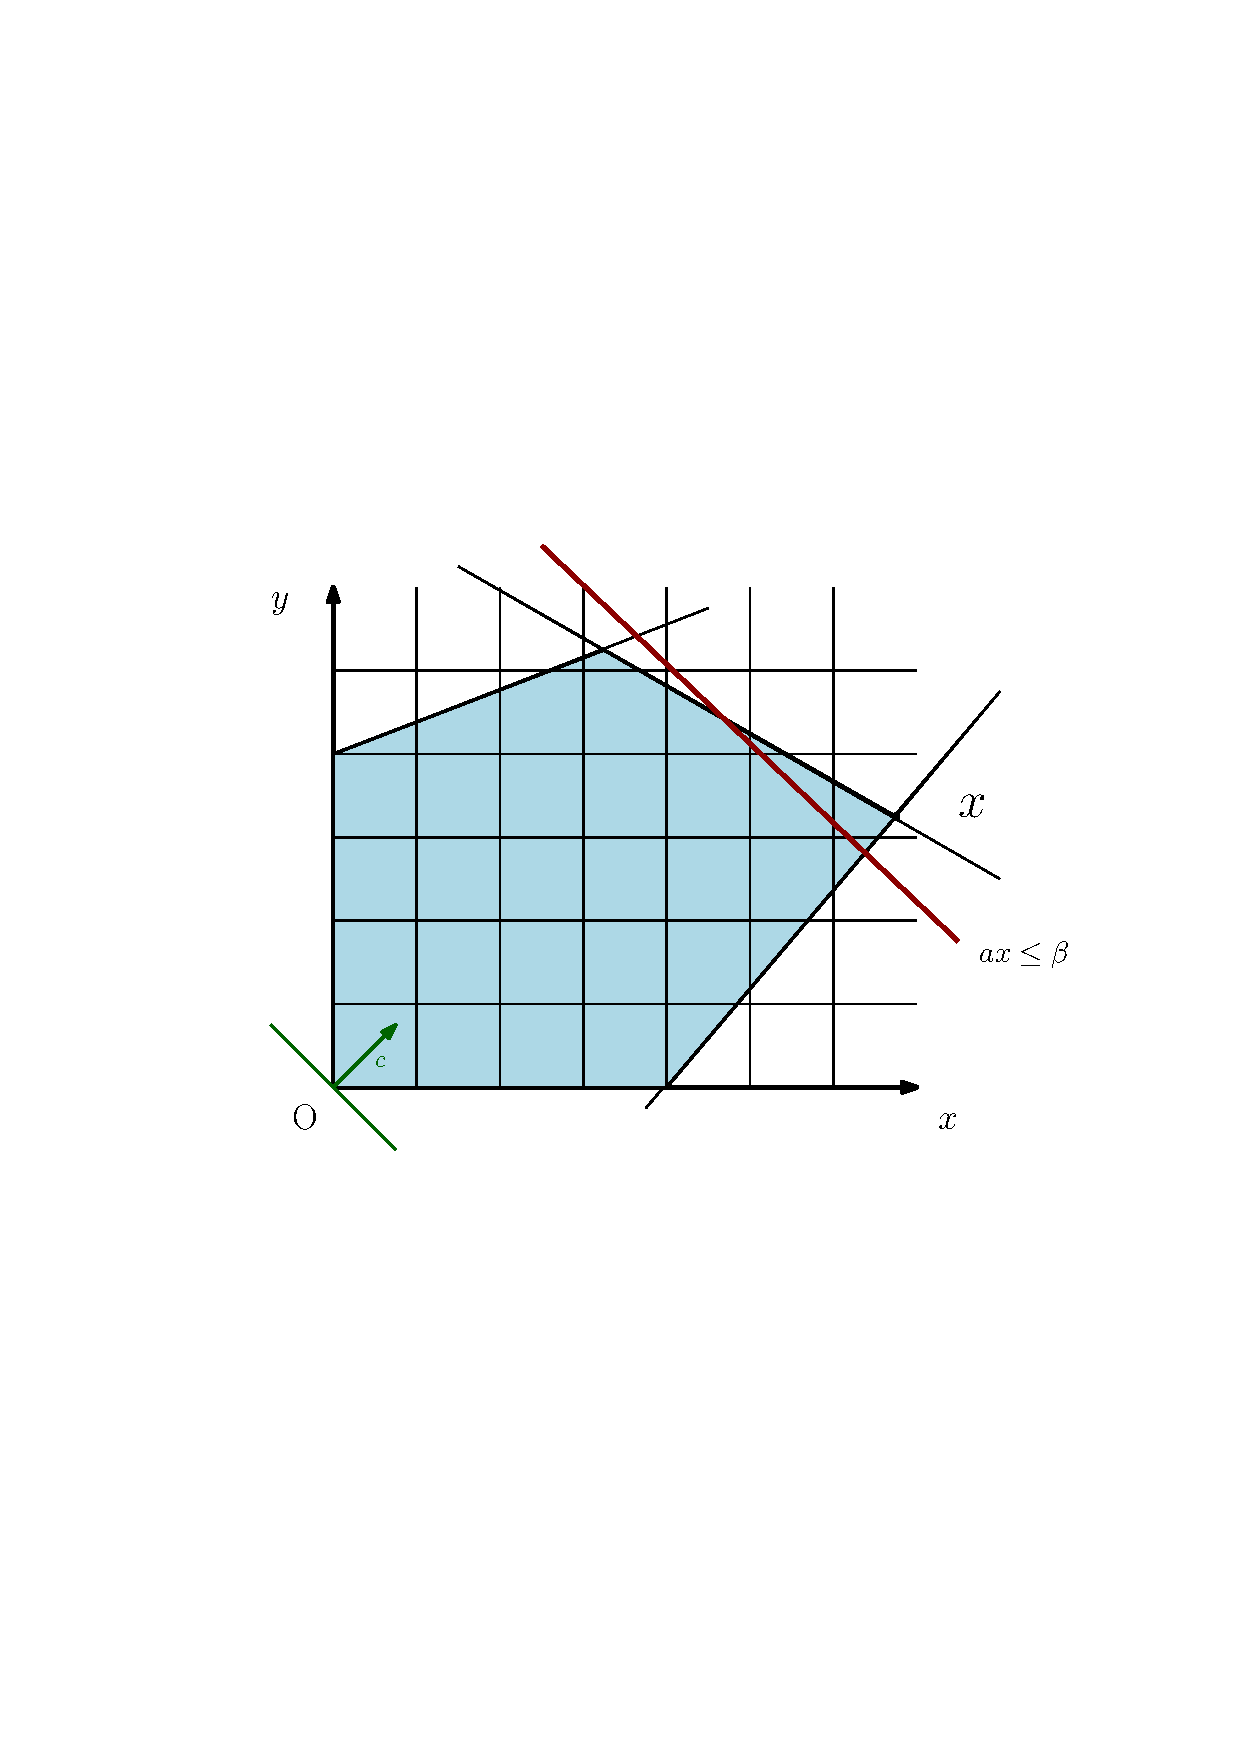
\includegraphics[width=0.6\linewidth]{anh2.pdf}
       
    \end{figure}
    \end{frame}

    \begin{frame}{ Ý tưởng phương pháp cắt của Danzig}
         Việc giải một bài toán $P^N$ là một quá trình gồm nhiều bước:\\
a) Ở bước thứ $r$,  giải bài toán bài toán quy hoạch tuyến tính phụ 
 $P_r, r = 0,1,... 
… \text{với}   F_0=F $\\
b) Tập các điểm  nguyên của tất cả các đa diện lồi là như nhau:
$$F_0^N=F_1^N=F_2^N=...=F_r^N=.......$$\\
Do đó, nếu phương án tối ưu $X^*_r$ của bài toán $P_r$ thoả mãn điều kiện nguyên thì nó cũng là phương án tối ưu $X_0$ của bài toán xuất phát $P^N_0$ và quá trình kết thúc.\\
\end{frame}

    \begin{frame}{ Ý tưởng phương pháp cắt của Danzig}
c)  Nếu $X^*_r$ không thoả mãn điều kiện nguyên thì $X^*_r$ không phải là 
phương án của bài toán $P_{r+1}$, tức là $X_r^*\notin F_{r+1}$.\\Chuyển từ bước $r$ sang bước $r+1$, tức là chuyển từ bài toán $P_r$ sang 
 $P_{r+1}$ khi $X^*_r$ không nguyên được thực hiện nhờ một lát cắt đúng $a_rx \le \beta_r$.\\
Việc bổ sung lát cắt này vào ràng buộc của bài toán $P_r$ sẽ chuyển đa diện lồi $F_r$ thành $F_{r+1}$.\\
    \end{frame}
\section*{Thuật toán Gomory cho bài toán nguyên hoàn toàn}
    \begin{frame}{Cơ sở lý thuyết}
        Ta xét bài toán tối ưu nguyên hoàn toàn:\\
\begin{equation}\label{Gomory1}
     \begin{split}
      (P^N) \quad    & {\rm{Max}} \langle c,x \rangle\\
          \rm{s.t} &\left\{\begin{split}
            & Ax= b,\\
           & x_j \ge 0, j=1,2,...,n.\\
            & x_j \text{nguyên}, j=1,2..,n.\\
           \end{split}\right.
       \end{split}
   \end{equation}
   \begin{dn}
     Giả  sử hệ véc-tơ $\{A^j,j\in J\}$ là cơ sở tương ứng với phương án cực biên ban đầu của bài toán $P^N$, các véc-tơ $A^j$ và các biến $x_j$ với $j\in J$ được gọi là các véc tơ cơ sở và biến cơ sở; còn các véc-tơ $A^j$ và các biến $x_j$ mà $j \notin J$ được gọi là các véc-tơ tự do và các biến tự do (biến phi cơ sở).\\  
   \end{dn}
    \end{frame}

    \begin{frame}{Cơ sở lý thuyết}
         Giả sử $X$ là phương án  tối ưu của bài toán $P^N$, từ đó ta có thể biểu diễn các biến cơ sở qua Các biến phi cơ sở:\\
   \begin{equation}\label{2.4}
       x_{i}=x_{i0} + \sum_{j \in N} x_{ij}(-x_j), i=\overline{0,m}.
   \end{equation}
    \end{frame}

    \begin{frame}{Cơ sở lý thuyết}
        \begin{dl}
        Giả sử $X$ có $x_{i0}$ không nguyên với $1\le i\le n$ và:\\
        1)\begin{equation}\label{2.5}
            z_i\equiv z_i(X)= -\{x_{i0}\} + \sum_{j \in \mathbb {N} }(-\{x_{ij}\})(-x_{j}), i=\overline{1,n}.
        \end{equation} \\
        2) $x$ là phương án của bài toán $P^N$.\\
        Khi đó:\\
        a) $z_i \hspace{0.1cm} \text{nguyên}$.\\
        b) $z_i \ge 0$. 
        \end{dl}
    \end{frame}

    \begin{frame}{Cơ sở lý thuyết}
        \begin{hq}
        Giả sử $X(L,C)$ không thoả mãn điều kiện nguyên, như vậy đối 
với $i$ nào đó $(1\le i \le 0) \hspace{0.1cm} x_{i0}$ không nguyên . Khi đó các hệ thức \eqref{2.5}  và $z_i \ge 0$ xác định một lát cắt đúng.
    \end{hq} 
    \end{frame}

    \begin{frame}{Dấu hiệu bài toán không có lời giải}
        \begin{figure}[h]
\centering
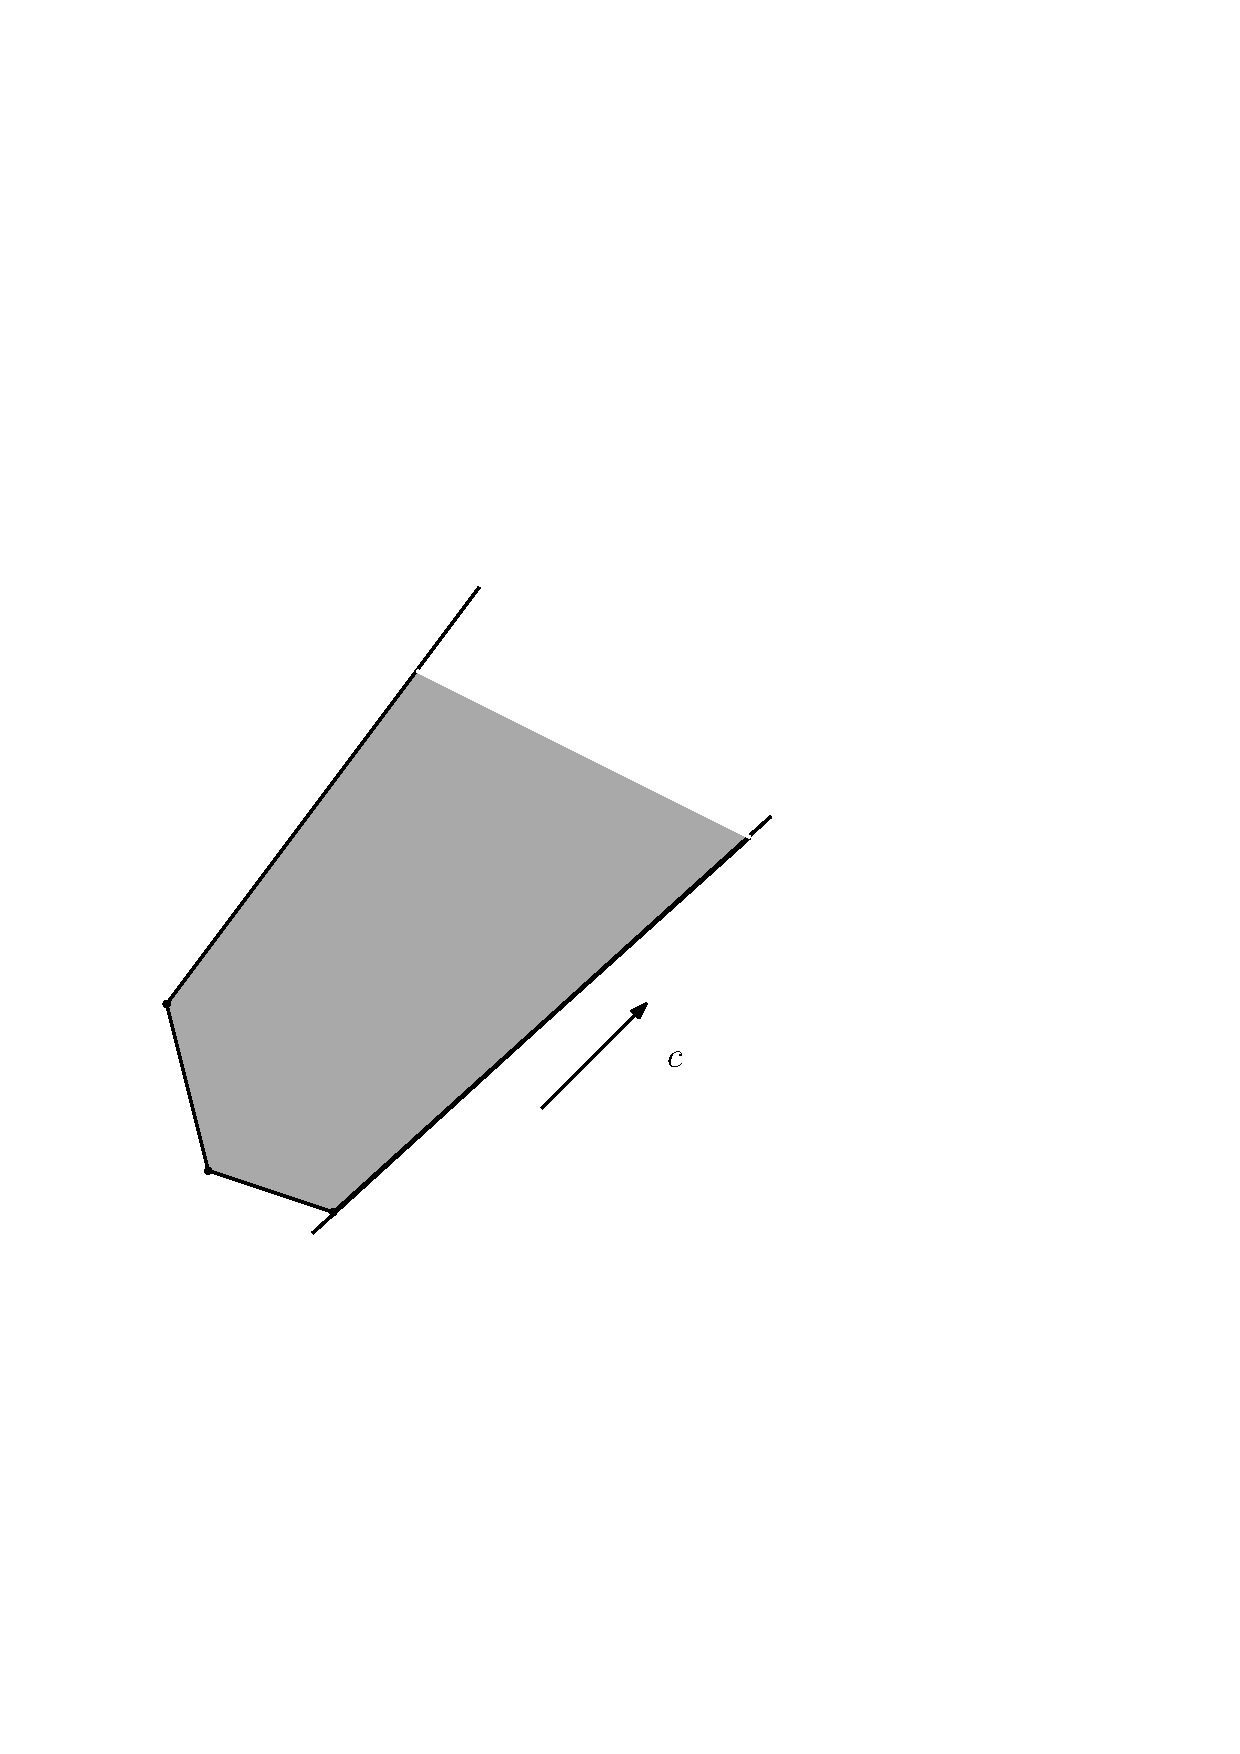
\includegraphics[width=0.45\linewidth]{anh3.pdf}
\caption{$\overline{P}$ không có lời giải}
\end{figure}
    \end{frame}

    \begin{frame}{Dấu hiệu bài toán không có lời giải}
        Về sau ta sẽ giả thiết:\\
1) Hàm mục tiêu $x_0\equiv CX$ bị chặn trên $F$.\\
2) Nếu tập hợp các phương án tối ưu của $P$ khác trống thì nó phải bị chặn, tức là nếu bài toán $P$ giải được thì bài toán $\overline{P}$ cũng giải 
được.\\
    \end{frame}

    \begin{frame}{Thuật toán Gomory}
        \textbf{Bước 1:}
Giải bài toán $P\equiv P_0$ đã cho bằng phương pháp đơn hình đối ngẫu.\\
- Nếu $P_0$ không giải được thì $P_0^N$ cũng không giải được.\\
- Nếu  $P_0$ giải được và nghiệm của nó thỏa mãn điều kiện nguyên thì nó cũng là phương án tối ưu của $P^N_0$, còn nếu chưa thỏa điều kiện thì chuyển sang bước 2.\\
       
    \end{frame}

    \begin{frame}{Thuật toán Gomory}
     \textbf{Bước 2:}
Chọn dòng đầu tiên ứng với thành phần không nguyên:\\
$k=min\{i|i\in \{1,...,n\},x_{i0}^r \text{không nguyên}\}$ và xây dựng lát cắt đúng:\\
$$   \begin{cases}\label{latcat}
    x_{n+r+1}= -\{x_{k0}^r\} + \sum_{j\in N_r}(-\{x_{kj}^r\} )(-x_j)\\
    x_{n+r+1} \ge 0\\
    x_{n+r+1} \hspace{0.1cm} \text{nguyên}
\end{cases}$$
Thêm lát cắt vào bảng đơn hình và tiếp tục giải bài toán $P^N_{r+1}$.\\
        \textbf{Bước 3:}
Sau khi tính toán với lát cắt nếu được phương án tối ưu thỏa mãn điều kiện nguyên thì thuật toán dừng lại. Nếu không thỏa mãn thì quay lại bước 2 cứ lần lượt như vậy thực hiện các bước lặp $r \ge 0$ cho đến khi thỏa mãn điều kiện.\\

    \end{frame}

     \begin{frame}{Tính hữu hạn của thuật toán}
         \begin{dl}
Giả sử có các điều kiện sau:\\
1) Tính nguyên của hàm mục tiêu $x_0\equiv CX$ được đảm bảo và $x_0$ được xét khi chọn dòng xây dựng lát cắt đúng.\\
2) Một trong các khẳng định sau là đúng:\\
i) Hàm mục tiêu $x_0$ bị chặn dưới trên $F_0$.\\ 
ii) Bài toán $P^N_0$ có ít nhất một phương án $X'$.\\
 Khi đó thuật toán Gomory thứ nhất kết thúc sau một số hữu hạn bước lặp lớn.
 \end{dl}
\end{frame}









\section{Phương pháp Land-Doig}



\section{Kết luận và Hướng phát triển}

\begin{frame}{Tài liệu tham khảo}
\end{frame}

%sample
\begin{frame}
\end{frame}

\begin{frame}
    \begin{block}{}
    \medskip
    \center{\huge \it \textcolor[rgb]{0.50,0.30,1.0}{Cảm ơn quý thầy cô và các anh chị đã quan tâm theo dõi!}}
    \medskip
    \end{block}	
\end{frame}    
\end{document}
